% !TEX root = main.tex
\chapter{Background}
\label{cha:background}
This chapter introduce basics of speech recognition related to this work.
Section~\ref{sec:back_asr} introduces speech preprocessing, \acf{AM} and \acf{LM} training, and explains important aspects of speech decoding.
Next sections describe specific speech recognition software implementations.
The~Kaldi toolkit is described in Section~\ref{sec:back_kaldi}, the~\ac{HTK} toolkit in Section~\ref{sec:back_htk} and the~Julius decoder in Section~\ref{sec:back_julius}.

The~statistical methods for continuous speech recognition were established more than 30 years ago. 
The~most popular statistical methods are based on acoustic modelling using \acp{HMM} and n-grams \acp{LM}, which are also used in Kaldi, the~toolkit of our choice.
We introduce principles of speech recognition and present techniques which are used in Kaldi. 

\begin{figure}[!htp]
    \begin{center}
    % Generated with LaTeXDraw 2.0.8
% Sun Jul 07 00:14:55 CEST 2013
% \usepackage[usenames,dvipsnames]{pstricks}
% \usepackage{epsfig}
% \usepackage{pst-grad} % For gradients
% \usepackage{pst-plot} % For axes
\scalebox{1} % Change this value to rescale the drawing.
{
\begin{pspicture}(0,-3.7639062)(9.26,3.7639062)
\usefont{T1}{ptm}{m}{n}
\rput(2.0,3.3){\psovalbox{Speech Input}}
\psline[linewidth=0.04cm,arrowsize=0.05cm 2.0,arrowlength=1.4,arrowinset=0.4]{->}(2.0,2.8)(2.0,2.3)
\usefont{T1}{ptm}{m}{n}
\rput(2.0454688,1.5789063){\psdblframebox[framesep=10pt]{Signal processing}}
\usefont{T1}{ptm}{m}{n}
\rput(2.0,0.3){\psovalbox{Acoustic observations $a$\tiny For example \acs{MFCC}}}
\psline[linewidth=0.04cm,arrowsize=0.05cm 2.0,arrowlength=1.4,arrowinset=0.4]{->}(2.0,0.9)(2.0,0.3)
\usefont{T1}{ptm}{m}{n}
\rput(2.0,-0.9){\psdblframebox[framesep=10pt]{Decoding $w^*$: \small $argmax_{w} P(a \mid w)*P(a)$}}
\usefont{T1}{ptm}{m}{n}
\rput(2.0,-1.6210938){}
\usefont{T1}{ptm}{m}{n}
\rput(8.5,-0.5){\psframebox{Language model: $P(w)$}}
\psline[linewidth=0.04cm,arrowsize=0.05cm 2.0,arrowlength=1.4,arrowinset=0.4]{<-}(5.8,-0.6)(6.3,-0.6)
\rput(8.7,-1.3){\psframebox{Acoustic model: $P(a \mid w)$}}
\psline[linewidth=0.04cm,arrowsize=0.05cm 2.0,arrowlength=1.4,arrowinset=0.4]{<-}(5.8,-1.2)(6.3,-1.2)
\usefont{T1}{ptm}{m}{n}
\rput(2.0, -2.4){\psovalbox{Recognized word $w^*$}}
\psline[linewidth=0.04cm,arrowsize=0.05cm 2.0,arrowlength=1.4,arrowinset=0.4]{->}(2.0,-1.5)(2.0,-1.9)
\end{pspicture} 
}

    \caption{Architecture of statistical speech recognizer\cite{ney1990acoustic}}
    \label{fig:components} 
    \end{center}
\end{figure}

\section{Automatic speech recognition}
\label{sec:back_asr}

The~goal of statistical \ac{ASR} is to decode the~most likely word sequence given speech.
The~term \term{decoding} finds its origin in \acs{HMM} terminology. 
In speech recognition it is equivalent to \term{recognizing} the~word sequence from the~speech. 
Formally, we search for the~most probable sequence of~words $w^*$ given the~acoustic observations $a$ as described in Equation~\ref{eq:best_fix}.
The~best word sequence $w^*$ does not depend on probability of the~acoustic features $P(a)$ so it can be eliminated as shown on the~second row of the~equation.

\begin{equation}\label{eq:best_fix}
    \begin{split}
    w^* = argmax_{w}\{P(w \mid a)\} &= argmax_{w}\{\frac{P(a \mid w) * P(w)}{P(a)}\} \\
                                    &= argmax_{w}\{P(a \mid w) * P(w)\}
    \end{split}
\end{equation}

The~task of acoustic modelling is to estimate the~parameters $\theta$ of a~model so the~probability $P(a \mid w ; \theta)$ is as accurate as possible.\footnote{Acoustic modelling is described in Section~\ref{sub:am}.} 
Similarly, the~\ac{LM} represents the~probability $P(w)$. \footnote{We describe language modelling in Section~\ref{sub:lm}.}

\ml{frames}
The~Figure~\ref{fig:components} illustrate the~process of decoding the~most probable word hypotheses $w^*$ for given speech utterance. 
First, the~sampled audio signal is processed by speech parametrisation and feature transformations, so the~decoding itself takes acoustic features $a$ as input. The~acoustic features $a$ are computed on small overlapping windows of audio signal.
The~acoustic signal in one windows is known as a~frame.

The~decoding itself is performed time synchronously frame by frame using beam search.
The~beam search expands hypotheses from previous step by taking account the~new frame features, and it computes probabilities of the~expanded hypotheses using \ac{AM} and \ac{LM}.
If the~number of hypotheses exceeds the~beam, the~low probable hypotheses are pruned.
% Pruning only the~least probable hypotheses may lead to discarding globally optimal hypotheses.
After the~decoding the~last audio frame, all hypotheses represents whole utterance.
The~word labels $w^*$ are extracted from the~most probably hypothesis which survived the~beam search.

Improving the~accuracy of speech recognition engine depends mainly on improving \ac{AM} and \ac{LM}
and also on parameters of the~beam search such as threshold how many hypotheses are allowed at maximum.


\subsection{Speech parameterisation}
\label{sub:param}
The~goal of speech parameterization is to reduce the~negative environmental influences on speech recognition.
The~speech varies in a~number of aspects. Some of them are listed below:
\begin{itemize}
    \item Differences among speakers pronunciation depends on gender, dialect, voice, etc.
    \item Environmental noises. In the~dialogue system Alex where our \ac{ASR} implementation is used the~speech is typically recorded in a~noisy street environment.
    \item The~recorded channel.
        For example the~telephone signal is reduced to frequency band between 300 to 3000Hz.
        The~quality of mobile phone signal also influences the~quality of the~audio signal.
\end{itemize}
Different speech parametrisation may improve robustness of speech recognition for different recording conditions.
% Note that speech parametrisation transformations the~acoustic signal based on few numerical parameters, which are constant for all recording conditions during training and decoding.
% Simply put, the~acoustic signal is transformed by boosting frequencies, which are informative for speech.

\ml{acoustic features}
Speech parametrisation extracts speech-distinctive acoustic features from raw waveform.
The~two most successful methods for speech parametrisation in last decades are \ac{MFCC}\cite{davis1980comparison} and \ac{PLP}\cite{hermansky1990perceptual}.
% change ti to something else than 
% SPEECH SIGNAL PARAMETERIZATION TECHNIQUES FOR SPEECHUNDERSTANDING SYSTEM Gaurav K. LEEKHA, Mrs. Meenakshi MEHLA, Shrilekha SAGWAL
Both \ac{MFCC} and \ac{PLP} transformations are applied on a~sampled and quantized audio signal.\footnote{In our experiments we use 16 kHz sampling frequency and 16 bit samples.} 
For each window \ac{MFCC} or \ac{PLP} efficiently computes statistics with a~reduced dimension. 
% The~sampling frequency is typically 8000, 16000 or 32000 Hz.
% Each sample is usually encoded to 8, 16 or 32 bits. 
The~methods are very computationally effective and significantly improve the~quality of recognised speech.

The~toolkits used in our dialogue system, Kaldi and \ac{HTK} toolkit, compute \ac{MFCC} coefficients for given audio input in a~similar way.\footnote{The~subtle differences are caused by implementation approaches, but does not effect the~quality of~\ac{MFCC} coefficients in~significant way.}
Therefore, we choose \ac{MFCC} as speech parametrisation technique for both toolkits, so we can compare them.

% An interested reader can find comprehensive introduction into signal processing 
% in~the~fourth Chapter of Spoken Language Processing book\cite{huang2001spoken}.

The~\ac{MFCC} statistics are computed for each frame.
In Figure~\ref{fig:mfcc_window} there are 7 windows --- frames with length of 25 ms and frame shift of 10 ms.
The~whole utterance lasts 85 ms.

\begin{figure}[!htp]
    \begin{center}
    ../../text/images/mfcc_window.tex
    \caption{\ac{PLP} or \ac{MFCC} features are computed every 10 ms seconds in 25 ms windows.
    Audio length is $(frames-1)*shift + win\_len = 85ms$}
    \label{fig:mfcc_window} 
    \end{center}
\end{figure}

Let us describe the~\ac{MFCC} computation for 25 ms window shifted by 10 ms and 16kHz audio sampling frequency. 
The~$16000 * 0.025 = 400$ samples in one window are reduced to 13 static cepstral coefficients.

The~\ac{MFCC} static features are usually extended by time derivatives $\Delta+\Delta\Delta$ features \cite{psutka2001comparison}.
As a~result, \ac{MFCC} $\Delta+\Delta\Delta$ extracts $13 + 13 + 13 = 39$ acoustic features for one frame. 
The~original vector of 400 audio samples in one frame is reduced to vector of 39 \ac{MFCC} $\Delta+\Delta\Delta$ acoustic features.

The~\ac{MFCC} features are computed by the~following steps:
{\small \begin{enumerate}
    \item The~audio samples are transformed into \term{frequency domain} by~\ac{DFT} in the~window.
    \item The~frequency spectrum from the~previous step is transformed onto the~mel scale, a~perceptual scale of frequencies, using triangular overlapping filters.
    \item From the~mel frequencies the~logs of the~powers are taken from each of the~mel frequencies.
    \item At the~end the~discrete cosine transform is applied on the~list of mel log powers.
    \item The~\ac{MFCC} coefficients are the~amplitudes of the~resulting spectrum.
    \item The~$\Delta+\Delta\Delta$ coefficients are computed from the~current and previous static features. See Figure~\ref{fig:delta}.
\end{enumerate}}

\begin{figure}
    \begin{center}
    ../../text/images/mfcc-delta.tex
    \caption{Typical setup with 39 features using \ac{MFCC}.}
    \label{fig:delta} 
    \end{center}
\end{figure}

\subsection*{Feature space transformations}
Feature space transformations are usually applied in addition to \ac{MFCC} or \ac{PLP} parametrisation.
\ml{frame}
The~feature space transformations are also typically applied per frame, but they usually take into account context of several preceding (left context) and consecutive frames (right context).

The~linear or affine transformations are expressed by matrix multiplications $Ax$ respectively $Ax^+$.
The~matrix $A$ represents the~transformation. 
The~$x$ is the~input vector and $Ax$ are the~transformed features.
The~affine transformations uses extended vector $(x^+)^T = (x_1, \ldots, x_n, 1)$ and matrix $A: (n+1)*(n+1)$.

There is a~large variety of available transformations. 
Dependently on acoustic data one should choose the~most appropriate one.
% The~transformations differ according to how they are estimated, namely for linear transformations how the~matrix $A$ is trained.
Some transformations are estimated discriminatively, some use generative models.
Some are speaker dependent, some speaker independent.

We list some of Kaldi transformations in order to illustrate rich choice of feature transformations in Kaldi toolkit.
% use and city http://kaldi.sourceforge.net/transform.html#transform_cmllr_global
\begin{itemize}
    \item \acf{HLDA}\cite{gales1999semi}.
    \item \acf{LDA}\cite{gopinath1998maximum} is typically used with \acs{MLLT} for speaker independent training.
    \item \acf{MLLT} also known as \acf{STC}\cite{gopinath1998maximum}
    \item \acf{ET}\cite{povey2011exponential}. It uses small number of speaker specific parameters for adaptation on speaker.
    \item \acf{CMVN}\cite{molau2003feature}. Typically normalise the~cepstrum mean and variance per speaker.
\end{itemize}

In our acoustic modelling scripts, see Chapter~\ref{cha:train},  we use two non-speaker adaptive feature transformations, which can be computed with very small context. 
The~first transformation, $\Delta+\Delta\Delta$  for \ac{MFCC} coefficients, was already introduced.
The~second transformation, \ac{LDA} and \ac{MLLT}, is described briefly below.

\subsubsection*{\acl{LDA} and \ac{MLLT} feature transformation}
The~\ac{LDA}+\ac{MLLT} is an alternative setup to $\Delta+\Delta\Delta$ transformation in our training scripts.
We use it also on top of \ac{MFCC} coefficients.
Using several spliced \ac{MFCC} vectors the~\ac{LDA}+\ac{MLLT} searches for the~best dynamic transformation.

The~combination of \ac{LDA} and \ac{MLLT} applies the~feature transformation in two steps: \ac{LDA} reduces the~feature dimension and \ac{MLLT} applies linear simple transformation\cite{gopinath1998maximum}.
Whereas, the~\ac{HLDA} estimates dimension reduction and space transformation in one step.\cite{gales1999semi}
The~combination \ac{LDA} and \ac{MLLT} performs very similar feature transformation to \ac{HLDA} and gains significant improvements over $\Delta+\Delta\Delta$ transformation similarly as \ac{HLDA}\cite{gales1999semi}\cite{gopinath1998maximum}.

% To conclude, the~signal processing samples the~continuous audio at regular interval intervals. 
% Fixed number of consecutive samples forms a~window. The~windows are usually overlapping.
% The~acoustic features are computed for each of the~overlapping window. 

\subsection{Acoustic modelling}
\label{sub:am}
Acoustic modelling is arguably the~heart of speech recognition.
The~\ac{AM} estimates the~probability $P(a|w; \theta)$ of generating acoustic features $a$ for given words $w$ and thus directly affects speech recognition quality as seen in~Equation~\ref{eq:best_fix}.

Acoustic modelling has only partial information available for training \ac{AM} parameters $\theta$ because the~corresponding textual transcription is time-unaligned.
The~hidden information of the~word (time) alignment in a~utterance makes acoustic model training more challenging.
Modern speech recognition toolkits use \acl{HMM} for modelling uncertainty between acoustic features and the~corresponding transcription. 

\subsubsection*{Choice of training units}
The~most successful acoustic modelling methods do not estimate the~$P(a|w)$ directly, but estimate probability $P(a|f_1f_2f_3f_4)$ of generating acoustic features $a$ for phones $w=f_1f_2f_3f_4$ which forms the~pronunciation of the~word $w$. Moreover, the~triphones are used even more successfully for estimating probability of acoustic features give word pronunciation.

\ml{phone}
Phone is the~smallest contrastive unit of speech. 
Let us see few examples of words and their phonetic transcriptions according CMU dictionary\cite{weide1998cmu}.
\begin{itemize}
    \item \term{youngest} \& \term{Y AH1 NG G AH0 S T}
    \item \term{youngman} \& \term{Y AH1 NG M AE2 N}
    \item \term{earned} \& \term{ER1 N D}
    \item \term{ear} with two transcribed pronunciations \term{IY1 R} and \term{IH1 R}
\end{itemize}
The~CMU dictionary distinguishes among several variations for each vowel e.g. \term{AH1} and \term{AH0}.
% It distinguishes the~pronunciation for \term{earned} and \term{ear} despite the~same transcription in the~first three letters.
It also stores two possible pronunciations for the~word \term{ear}.

The~acoustic features for a~phone significantly depend on its~context.
The~previous and the~following phone strongly influence the~sound of the~middle phone.

\ml{triphone}
The~triphone is a~sequence of three phones and captures the~context of single phone.
As a~result, acoustic properties of the~triphones vary much less according to the~context than phones.
Let us note that certain combinations of prefixes have the~same effect on the~central phone,
e.g. \term{q} and \term{k} has the~same effect on \term{i}. % cite??
In order to reduce the~number of triphones for acoustic modelling, these triphones are clustered together.

% The~advantage of training triphone-\ac{AM} over word-\ac{AM} 
% is due to words sparsity. 
% There is typically less clustered triphones and many words for training data,
% so a~triphone model can be trained from much more examples than a~word model. 

% TODO mentioned curse of dimensionality for words -> more parameters than triphones for less examples

% \begin{figure}[!htp]
%     \begin{center}
%     % Generated with LaTeXDraw 2.0.8
% Fri Jul 05 23:18:35 CEST 2013
% \usepackage[usenames,dvipsnames]{pstricks}
% \usepackage{epsfig}
% \usepackage{pst-grad} % For gradients
% \usepackage{pst-plot} % For axes
\scalebox{1} % Change this value to rescale the drawing.
{
\begin{pspicture}(0,-2.54)(5.46,2.54)
\psframe[linewidth=0.04,dimen=outer](5.46,2.54)(2.92,1.76)
\psframe[linewidth=0.04,dimen=outer](2.44,2.54)(0.24,1.68)
\psframe[linewidth=0.04,dimen=outer](4.44,0.6)(1.08,-0.28)
\usefont{T1}{ptm}{m}{n}
\rput(1.3757813,2.205){Input}
\usefont{T1}{ptm}{m}{n}
\rput(4.1971874,2.165){Desired output}
\usefont{T1}{ptm}{m}{n}
\rput(2.6715624,1.18){\Huge +}
\psline[linewidth=0.04cm,arrowsize=0.05291667cm 2.0,arrowlength=1.4,arrowinset=0.4,doubleline=true,doublesep=0.12]{->}(2.66,-0.46)(2.66,-1.34)
\psframe[linewidth=0.04,dimen=outer](5.3,-1.56)(0.0,-2.54)
\usefont{T1}{ptm}{m}{n}
\rput(2.433125,-1.995){Data model}
\usefont{T1}{ptm}{m}{n}
\rput(2.85375,0.205){Training Algorithm}
\end{pspicture} 
}


%     % Generated with LaTeXDraw 2.0.8
% Sat Jul 06 10:26:19 CEST 2013
% \usepackage[usenames,dvipsnames]{pstricks}
% \usepackage{epsfig}
% \usepackage{pst-grad} % For gradients
% \usepackage{pst-plot} % For axes
\scalebox{1} % Change this value to rescale the drawing.
{
\begin{pspicture}(0,-2.41)(5.4382815,2.41)
\psframe[linewidth=0.04,dimen=outer](5.38,2.39)(2.96,1.31)
\psframe[linewidth=0.04,dimen=outer](2.8582811,2.41)(0.0,1.31)
\psframe[linewidth=0.04,dimen=outer](4.64,0.57)(0.9382811,-0.31)
\usefont{T1}{ptm}{m}{n}
\rput(1.4256251,1.935){Mfcc coeficients}
\usefont{T1}{ptm}{m}{n}
\rput(4.0285935,2.075){Text}
\usefont{T1}{ptm}{m}{n}
\rput(2.7729685,0.87){\Huge +}
\psline[linewidth=0.04cm,arrowsize=0.05291667cm 2.0,arrowlength=1.4,arrowinset=0.4,doubleline=true,doublesep=0.12]{->}(2.7982812,-0.45)(2.7982812,-1.33)
\psframe[linewidth=0.04,dimen=outer](5.4382815,-1.43)(0.1382812,-2.41)
\usefont{T1}{ptm}{m}{n}
\rput(2.579375,-1.865){Acoustic model}
\usefont{T1}{ptm}{m}{n}
\rput(2.7045312,0.175){Baum-Welsh Algorithm}
\usefont{T1}{ptm}{m}{n}
\rput(1.4325,1.63){\footnotesize Extracted from audio}
\usefont{T1}{ptm}{m}{n}
\rput(4.2509375,1.63){\footnotesize Transcribed audio}
\end{pspicture} 
}

%     \caption{Supervised learning idea and example}
%     \label{fig:supervised} 
%     \end{center}
% \end{figure}

\subsubsection*{\acfp{HMM}}
The~\acp{HMM} is a~very powerful statistical method for~characterizing observed data samples of~a~discrete-time series with an unknown state. \cite{huang2001spoken}. % huang2001spoken chapter 8
In case of speech recognition the~hidden states typically represent monophones or triphones and we observe samples of the~acoustic features.

\ml{transition probability}
Hidden Markov Models have two type of parameters \term{transition probabilities among states} and \term{probabilistic distribution for generating observation in given state}.
These parameters need to be estimated in \ac{AM} training.\footnote{Both kind of parameters are denoted together as $\theta$ in Equation~\ref{eq:best_fix}.}

The~transition probability is a~probability of changing state $q$ to state $u$.
Each transition is represented as arc $e=qu$ between the~states $q$ and $u$, see~\ref{fig:hmm_words}.
The~probability is typically represented as the~weight $w_e$ of arc $e$.

Importantly, an \ac{HMM} use self loop arc $e=uu$ for all states to model acoustic features which are generated several times from the~same state $u$.
As a~result, an \ac{HMM} is able to model variable length of phones.

% For every node in a~Markov model must hold that the~sum weights of outgoing arcs is one.

\ml{Gaussian HMM}
The~Markov model emits an observation during traversal over its arcs.
The~\acl{HMM} emits the~observation stochastically based on the~probabilistic distribution related to~the~visited state.
In speech recognition, a~multivariate Gaussian distribution is typically used to model observation probabilities of \ac{HMM} states.
The~Gaussian distribution models probability of emitting acoustic features in given state.
The~parameters of the~Gaussian distribution are estimated for each state individually.
However, the~states are usually clustered during \ac{AM} training and the~states within a~cluster share same parameters to the~Gaussian distribution.


\subsubsection*{Training \ac{HMM}}
\label{sub:trainhmm}

The~Kaldi uses Viterbi training and the~\ac{HTK} toolkit uses \acl{EM} algorithms to train \ac{HMM} \acl{AM}.
The~toolkits models the~observation probabilities using multivariate Gaussian distribution with dimension of the~acoustic features $a$.
% Both Viterbi training and the~\ac{EM} algorithm starts with \ac{HMM} with initial values. 

Typically, the~transition probabilities are initialised with values uniformly distributed.
The~observation probabilities are usually initialized by multivariate Gaussian distribution with $\mu$ and $\Sigma$ set to global mean and global covariance matrix estimated on all training acoustic data.

\ml{EM}
Let us describe how the~\ac{EM} algorithm operates for one pair of training data consisting of acoustic features $a$ and corresponding text speech transcription $t$.
We create \ac{HMM} $t'$, where each state represents one monophone.\footnote{We describe the~identical training procedure for simplicity on monophones. The~state-of-the-art \acp{AM} use triphones.} 
The~monophones are extracted from transcription $t$ using pronunciation dictionary.
In Figure~\ref{fig:hmm_words} the~utterance \term{how do you do} was expanded to monophone \ac{HMM} model.
Given the~\ac{HMM} model for transcription $t$ and acoustic features $a$ the~parameters of the~model are estimated.
It should be obvious that only states representing phones in transcription can be trained by training pair $(a, t)$.
Consequently, one needs lot of training data to robustly estimate parameters of all states.

The~\ac{EM} algorithm iterates following steps in order to update parameters of transition and observation probabilities:
\begin{itemize}
    \item The~observation probabilities are computed using \ac{HMM} $t'$. 
    \item {\bf E-step}: Based on the~observation probabilities the~observation are align to states of \ac{HMM} $t'$. 
    \item {\bf M-step}: Based on the~alignment of observation to states the~$t'$ parameters are re-estimated. 
\end{itemize}

\ml{Baum-Welch}
The~{\bf E-step} finds a~distribution for the~alignment between \ac{HMM} $t'$ and transcription $t$ using \ac{MLE}\cite{gopinath1998maximum} and observation probabilities.
\ac{MLE} takes into account takes into account all possible alignments and its probabilities to compute the~resulting distribution.
The~Baum-Welch equations can be derived from the~fact, that the~\ac{MLE} criterion is also used for finding the~most probable distribution in {\bf M-step}.\cite{huang2001spoken}
% This variation of \ac{EM} algorithm for estimating \ac{HMM} parameters is called Baum-Welch algorithm.

\begin{figure}[!htp]
    \begin{center}
    % \usepackage[usenames,dvipsnames]{pstricks}
% \usepackage{epsfig}
% \usepackage{pst-grad} % For gradients
% \usepackage{pst-plot} % For axes
\scalebox{1} % Change this value to rescale the drawing.
{
\begin{pspicture}(5,2)
\usefont{T1}{ptm}{m}{n}
\rput(2.5,1){TODO HMM: how SIL are SIL you}
\end{pspicture} 
}

    \caption{Markov monophone model for four words. Such an \ac{HMM} is constructed for monophone Viterbi training and reference transcriptions \textit{how do you do}. The~parameters of the~\ac{HMM} model are updated according Equation~\ref{eq:mean},~\ref{eq:var} and~\ref{eq:weights}.}
    \label{fig:hmm_words} 
    \end{center}
\end{figure}

\subsubsection*{\acl{MLE} method}
\label{sub:mle_method}
The~\ac{MLE} is a~general approach to setting statistical model parameters.
It searches for best parameters $\theta^*$ in order to maximize the~likelihood function $f$ for \ac{IID} training data illustrated in Equation~\ref{eq:maxlikelihood}.
For \ac{IID} training data holds Equation~\ref{eq:lmjoint} describing data joint probability. 
\begin{equation}\label{eq:lmjoint}
    f(x_1, x_2, x_3, \ldots, x_n | \theta) = f(x_1 | \theta) * f(x_2 | \theta) * \ldots * f(x_n | \theta)
\end{equation}
The~likelihood function can be derived from Equation~\ref{eq:lmjoint} assuming training data fixed and parameter $\theta$ free as described in Equation~\ref{eq:likelihood}.
\begin{equation}\label{eq:likelihood}
    \mathcal{L}(\theta\,|\,x_1,\ldots,x_n) = \sum_{i=1}^n log(f(x_i|\theta))
\end{equation}
\begin{equation}\label{eq:maxlikelihood}
    \theta^* = argmax_{\theta} \mathcal{L}(\theta\,|\,x_1,\ldots,x_n)
\end{equation}

\subsubsection*{Viterbi training of acoustic models}
On the~other hand, the~Kaldi toolkit applies the~Viterbi criterion in assigning the~acoustic observation to \ac{HMM} states.
The~Viterbi training approximates \ac{EM} algorithm by choosing single best alignment and maximizing the~posterior probability for the~chosen alignment.
Latest work suggest that Viterbi training is just as effective for continuous speech recognition as Baum-Welch algorithm \cite{rodriguez2003comparative}.
Moreover, Viterbi training needs much less computational resources. 

We detail the~Viterbi training since it is used in the~Kaldi toolkit for acoustic model training and also a~very similar algorithm is used for Viterbi decoding.

Given set of training observations $O^r, 1 \le r \le R$ and \ac{HMM} state sequence $1<j< N$ the~observation sequence is aligned to the~state sequence via Viterbi alignment.\cite{buthpitiya2012parallel}
The~best alignment $T$ results from maximising Equation~\ref{eq:vit_align} for $1<i< N$.

\begin{equation}\label{eq:vit_align}
    \phi_N(T)= max_i[\phi_i(T)a_{iN}] 
\end{equation}

% \todo{describe T and T versus $o_t$}
% \todo{Should I cite every equation?}

The~$\phi_i(o_t)$ from Equation~\ref{eq:vit_align} is computed recursively according Equation~\ref{eq:state_prob}

\begin{equation}\label{eq:state_prob}
    \phi_i(o_t) = b_j(o_t) max \left\{
  \begin{array}{lr}
      \phi_j(t-1)a{jj}\\
      \phi_{j-1}(t-1)a{j-1j}
  \end{array}
\right.
\end{equation}

The~initial conditions are $\phi_1(1)=1$ and $\phi_j(1)= a_{1j}b_j(o_1)$, for $ 1 < j < N$.
In our case the~likelihoods are modeled as mixture Gaussian densities, so the~output probability $b_j(o_t)$ is defined as in Equation~\ref{eq:observ_prob}.

\begin{equation}\label{eq:observ_prob}
    b_j(o_t) = \sum_{m=1}^{M_j}{c_{jm}\mathcal{N}(o_t; \mu_{jm}, \Sigma_{jm})}
\end{equation}

The~$M_j$ represents number of mixture components in state $j$, $c_{jm}$ is the~weight of $m^{th}$ component and $\mathcal{N}(o_t; \mu_{jm}, \Sigma_{jm})$
is multivariate Gausian with mean vector $\mu$ and covariance $\Sigma$.

Firstly, model parameters are updated based on the~single-best alignment of individual observation to states and Gaussian components within states.
Secondly, transition probabilities are estimated from the~relative frequencies, Equation~\ref{eq:freq} where $A_{ij}$ denotes the~number of transitions from state $i$ to state $j$.

\begin{equation}\label{eq:freq}
    \hat{a}_{ij} = \frac{A_{ij}}{\sum_{k=2}^{N}{A_{ik}}}
\end{equation}

The~indicator function $\psi^r_{jm}(t)$ is used for updating means and covariance matrix from statistics.
It returns one if $o^r_t$ is associated with mixture component $m$ of state $j$ and is zero otherwise.
The~mean vector and covariance matrix is updated according Equations~\ref{eq:mean} and~\ref{eq:var}.

\begin{equation}\label{eq:mean}
    \hat{\mu_{jm}} = \frac{\sum_{r=1}^{R}{\sum_{t=1}^{T_r}{\psi^r_{jm}(t)o^r_t}}}  {\sum_{r=1}^{R}{\sum_{t=1}^{T_r}{\psi^r_{jm}(t)}}}
\end{equation}

\begin{equation}\label{eq:var}
    \hat{\Sigma_{jm}} = \frac{\sum_{r=1}^{R}{\sum_{t=1}^{T_r}{\psi^r_{jm}(t)(o^r_t - \hat{\mu_{jm}})(o^r_t - \hat{\mu_{jm}})'}}}  {\sum_{r=1}^{R}{\sum_{t=1}^{T_r}{\psi^r_{jm}(t)}}}
\end{equation}

Finally, the~mixture weights are computed based on the~number of observations allocated to each component.\footnote{The~Viterbi equations has the~same notation as in \cite{buthpitiya2012parallel}.}

\begin{equation}\label{eq:weights}
    c_{jm} = \frac{\sum_{r=1}^{R}{\sum_{t=1}^{T_r}{\psi^r_{jm}(t)}}} {\sum_{r=1}^{R}{\sum_{t=1}^{T_r}\sum_{l=1}^{M}{\psi^r_{jl}(t)}}}
\end{equation}


\ml{generative training}
To conclude, \ac{AM} are trained using \ac{MLE} or Viterbi training, which approximates the~theoretically optimal \ac{MLE} Baum-Welch training; however, in practice Viterbi training performs as well as \ac{MLE} modelling.
Baum-Welch or Viterbi training aim at modelling likelihood of spoken utterance and perform so called generative training.
However, discriminative methods, which re-estimates generative \acp{AM}, perform better.

\subsubsection*{Discriminative training}
\label{sub:subsection_name}
% subsection subsection_name (end)
\ml{discriminative training}
The~discriminative training uses its objective function and likelihood of generative models to discriminate -- boost differences between high probable and low probable hypotheses.
The~discriminative training is typically initialised by acoustic generative model from Baum-Welch or Viterbi training.
Then, the~likelihood from the~generative model is boosted according an objective function and the~\ac{AM} is re-estimated.
Following objective functions and accordingly named discriminative training methods are used in our training scripts:
\begin{itemize}
    \item \acl{MMI}\cite{chow1990maximum} 
        % Note the~\ac{MMI} function is implemented as \acs{bMMI} with boosted parameter set to 0.
    \item \acl{bMMI}\cite{povey2008boosted}
    \item \acl{MPE}\cite{povey2003mmi}
\end{itemize}
For details how the~methods are initialized and its usage in Kaldi see Chapter~\ref{cha:train}.

\subsection{Language modelling}
\label{sub:lm}

A~\acl{LM} effectively reduces and more importantly prioritise the~\ac{AM} hypothesis.
A~probability of acoustic features given words transcription $P(a|w)$ estimated by \ac{AM} is combined with the~probability of the~words transcription $P(w)$ estimated by \ac{LM} for given domain in order to compute posterior probability of transcription $P(w|a) = \frac{P(a|w)*P(w)}{P(a)}$.

The~statistical \ac{LM} assigns a~given word sequence its probability according Equation~\ref{eq:lm}.
The~most used, n-gram \acp{LM} compute the~probability of $k$ word sequence $W$ according Equation~\ref{eq:lm}.\cite{brants2007large}
The~Markov assumption approximates the~probability by assuming that only the~most recent $n-1$ words are relevant when predicting next word.
\ml{\ac{LM} order}
We call the~number $n$ an order of \ac{LM}.

\begin{equation} \label{eq:lm}
    P(W)=P(w_k,  w_{k-1}, w_{k-2}, ..., w_1) \approx \prod_{i=1}^{k}{P(w_i|w^{i-1}_{i-n+1})}
\end{equation}

The~probabilities $P(w_i|w^{i-1}_{i-n+1})$ for each word $w_i$ are estimated using relative frequencies of the~n-grams, (n-1)-grams, (n-2)-grams, \ldots on training data.
The~\ac{MLE} is used for estimating estimating relative frequencies $r$ according Equation~\ref{eq:freq}.
\begin{equation} \label{eq:freq}
    r(w_i|w^{i-1}_{i-n+1}) = \frac{f(w^i_{i-n+1})} {f(w^{i-1}_{i-n+1})}
\end{equation}
The~Equation~\ref{eq:freq} is intuitive but many valid and even reasonable utterances are missing or too few.
Consequently, the~numerator might be zero and the~relative frequency may be undefined.
\ml{sparse data}
This is known as sparse data problem.
\ml{LM smoothing}
Smoothing techniques are often used to estimate the~higher n-gram relative frequencies based on the~lower frequencies.\cite{goodman2001bit}.
In principle, the~predictive accuracy of the~language model can be improved by increasing the~order of the~n-gram.
However, doing so further exacerbates the~sparse data problem.\cite{brants2007large}

The~\ac{LM} estimates the~probability by counting the~relative frequencies on text corpus which is typically chosen according the~targeted \ac{ASR} domain.
For example, in training scripts which are described in Chapter~\ref{cha:train} we train the~\ac{LM} only on text transcriptions from the~training data using Witten-Bell smoothing.\cite{witten1991zero}


\subsection{Speech decoding}
\label{sub:decode}
The~speech \ac{HMM} decoders find the~most probable word sequences by searching phone sequences which corresponds to the~words.
The~phones are typically represented as triphones in \ac{AM}.

Using combination of \ac{AM} and \ac{LM} probabilities as described in~Equation~\ref{eq:best_fix} does not produce the~most accurate speech transcriptions. 
Typically a~\ac{LMW} $w_{lm}$ is used to improve speech recognition accuracy.
It is tuned on development set and balances the~impact of the~two models.
Using the~\ac{LMW} the~words best sequence is found according Equation~\ref{eq:am_lm}.

\begin{equation}\label{eq:am_lm}
    w^* = argmax_{w}\{P(w \mid a)\} = argmax_{w}\{P(a \mid w) * P(w)^{w_{lm}}\}
\end{equation}

The~\ac{ASR} is a~pattern recognition task as well as a~search problem.
In speech recognition, making a~search decision is also referred to as decoding.\cite{huang2001spoken}

For a~word recognition the~\ac{AM} limits the~possible phone sequences only to words in lexicon --- the~words in training data.
The~word recognition is nowadays the~most successful form of \ac{ASR}.
The~\ac{HMM} sequences represent phone sequence which forms words only as illustrated on Figures~\ref{fig:hmm_lm} and~\ref{fig:hmm_alt}.
The~words are connected via \ac{HMM} model which represent inter word silence.

For isolated word recognition the~\acp{HMM} are evaluated for each word possibility.
Using the~forward algorithm for each \ac{HMM} $h_w$, we are able to compute the~probability of every word $w$ given the~acoustic observations.
The~isolated word recognition becomes a~simple recognition problem, where we select the~most probable \ac{HMM} $h^*$ from a~finite set of word \acp{HMM}.

Note that the~\ac{HMM} training is identical for continuous \ac{ASR} and isolated word recognition,
but the~decoding is more complicated for continuous \ac{ASR} where we aim to decode word sequences.

\begin{figure}[!htp]
    \begin{center}
        % Generated with LaTeXDraw 2.0.8
% Sun Jul 07 00:14:55 CEST 2013
% \usepackage[usenames,dvipsnames]{pstricks}
% \usepackage{epsfig}
% \usepackage{pst-grad} % For gradients
% \usepackage{pst-plot} % For axes
\scalebox{1} % Change this value to rescale the drawing.
{
\begin{pspicture}(0,-5.0)(9.0,1.0)
\usefont{T1}{ptm}{m}{n}
\rput(4.5,0.5){\psdblframebox[framesep=10pt]{two}}
\rput(4.5,-2.5){\psdblframebox[framesep=10pt]{one}}

\psline[linewidth=0.04cm,arrowsize=0.05291667cm 2.0,arrowlength=1.4,arrowinset=0.4]{->}(0.9,-0.4)(3.7,0.5)
\psline[linewidth=0.04cm,arrowsize=0.05291667cm 2.0,arrowlength=1.4,arrowinset=0.4]{->}(0.9,-0.4)(3.7,-2.5)
\psline[linewidth=0.04cm,arrowsize=0.05291667cm 2.0,arrowlength=1.4,arrowinset=0.4]{->}(5.3,0.5)(8.0,-0.4)
\psline[linewidth=0.04cm,arrowsize=0.05291667cm 2.0,arrowlength=1.4,arrowinset=0.4]{->}(5.3,-2.5)(8.0,-0.4)
\rput(4.5,-4.5){sil}
\rput(2.3,0.5){$\epsilon$:$P(w_{two})$}
\rput(2.0,-2.1){$\epsilon$:$P(w_{one})$}
\rput(6.3,0.3){$\epsilon$}
\rput(6.3,-1.2){$\epsilon$}

\rput(0.5,-0.4){s}
\pscircle[linewidth=0.04,dimen=outer](0.5,-0.4){0.48}
\rput(8.5,-0.4){e}
\pscircle[linewidth=0.04,dimen=outer](8.5,-0.4){0.48}
\psarc[linewidth=0.04,linestyle=dashed,dash=0.16cm 0.16cm,tbarsize=0.07055555cm 5.0,arrowsize=0.1cm 2.0,arrowlength=1.4,arrowinset=0.4]{<-}(4.6,-0.9){4.00}{180.0}{360.0}
\end{pspicture} 
}

        \caption{Diagram of how \ac{LM} is combined with \acp{HMM}.}
        \label{fig:hmm_lm} 
    \end{center}
\end{figure}

Let us introduce simple example of continuous word \ac{ASR}.
Imagine a~\ac{LM} of order 1 modelling only two words - \term{one} and \term{two} each uniformly distributed\footnote{If a~\ac{LM} of order 1 assigns to every word equal probability, we say it has order 0}.
We want to decode any possible sequence of words \term{one}, \term{two}. 
The~$\epsilon$ transition at the~end of words \acp{HMM} to final state $e$ allow us introduce \ac{HMM} silence model which connect the~final state $e$ and start state $s$. 
Consequently, the~words are chained using silence \ac{HMM} model as illustrated in Figure~\ref{fig:hmm_lm}.
Expanded monophone \ac{HMM} for words \term{one} and \term{two} is shown in Figure~\ref{fig:hmm_alt}.
Note that \ac{LM} weight $P(w)$ can be stored on the~in the~$\epsilon$ transition at the~beginning.

\begin{figure}[!htp]
    \begin{center}
        % Generated with LaTeXDraw 2.0.5
% Wed Feb 19 14:58:50 CET 2014
% \usepackage[usenames,dvipsnames]{pstricks}
% \usepackage{epsfig}
% \usepackage{pst-grad} % For gradients
% \usepackage{pst-plot} % For axes
\scalebox{1} % Change this value to rescale the drawing.
{
\begin{pspicture}(0,-4.3059373)(9.08,4.33)
\pscircle[linewidth=0.04,dimen=outer](6.16,0.7940625){0.48}
\pscircle[linewidth=0.04,dimen=outer](3.86,0.7740625){0.48}
\psline[linewidth=0.04cm,arrowsize=0.05291667cm 2.0,arrowlength=1.4,arrowinset=0.4]{->}(4.32,0.7940625)(5.72,0.7740625)
\pscustom[linewidth=0.04]
{
\newpath
\moveto(3.86,0.3140625)
\lineto(3.83,0.1840625)
\curveto(3.815,0.1190625)(3.795,-0.0159375)(3.79,-0.0859375)
\curveto(3.785,-0.1559375)(3.775,-0.2659375)(3.77,-0.3059375)
\curveto(3.765,-0.3459375)(3.76,-0.4159375)(3.76,-0.4459375)
\curveto(3.76,-0.4759375)(3.76,-0.5159375)(3.76,-0.5259375)
}
\pscustom[linewidth=0.04]
{
\newpath
\moveto(3.5,-0.1459375)
\lineto(3.55,-0.2359375)
\curveto(3.575,-0.2809375)(3.62,-0.3509375)(3.64,-0.3759375)
\curveto(3.66,-0.4009375)(3.7,-0.4509375)(3.72,-0.4759375)
}
\pscustom[linewidth=0.04]
{
\newpath
\moveto(3.98,-0.1859375)
\lineto(3.9,-0.2559375)
\curveto(3.86,-0.2909375)(3.8,-0.3459375)(3.78,-0.3659375)
}
\pscustom[linewidth=0.04]
{
\newpath
\moveto(6.14,0.2940625)
\lineto(6.11,0.1640625)
\curveto(6.095,0.0990625)(6.075,-0.0359375)(6.07,-0.1059375)
\curveto(6.065,-0.1759375)(6.055,-0.2859375)(6.05,-0.3259375)
\curveto(6.045,-0.3659375)(6.04,-0.4359375)(6.04,-0.4659375)
\curveto(6.04,-0.4959375)(6.04,-0.5359375)(6.04,-0.5459375)
}
\pscustom[linewidth=0.04]
{
\newpath
\moveto(5.78,-0.1659375)
\lineto(5.83,-0.2559375)
\curveto(5.855,-0.3009375)(5.9,-0.3709375)(5.92,-0.3959375)
\curveto(5.94,-0.4209375)(5.98,-0.4709375)(6.0,-0.4959375)
}
\pscustom[linewidth=0.04]
{
\newpath
\moveto(6.26,-0.2059375)
\lineto(6.18,-0.2759375)
\curveto(6.14,-0.3109375)(6.08,-0.3659375)(6.06,-0.3859375)
}
\usefont{T1}{ptm}{m}{n}
\rput(3.48,-0.8359375){T}
\usefont{T1}{ptm}{m}{n}
\rput(5.933125,-0.8959375){UW1}
\rput{-6.2}(-0.14201093,0.4346221){\psarc[linewidth=0.04,arrowsize=0.013cm 5.43,arrowlength=1.06,arrowinset=0.46]{->}(3.9415283,1.5283893){0.31510985}{296.34583}{245.37376}}
\rput{-6.2}(-0.13276115,0.6854146){\psarc[linewidth=0.04,arrowsize=0.013cm 5.43,arrowlength=1.06,arrowinset=0.46]{->}(6.2615285,1.5683894){0.31510985}{296.34583}{245.37376}}
\pscircle[linewidth=0.04,dimen=outer](8.6,-0.4059375){0.48}
\psline[linewidth=0.04cm,arrowsize=0.05291667cm 2.0,arrowlength=1.4,arrowinset=0.4]{->}(6.56,0.5740625)(8.16,-0.3459375)
\psline[linewidth=0.04cm,arrowsize=0.05291667cm 2.0,arrowlength=1.4,arrowinset=0.4]{->}(0.88,-0.4459375)(3.44,0.7140625)
\pscircle[linewidth=0.04,dimen=outer](3.34,-2.3859375){0.48}
\pscircle[linewidth=0.04,dimen=outer](5.14,-2.4459374){0.48}
\psline[linewidth=0.04cm,arrowsize=0.05291667cm 2.0,arrowlength=1.4,arrowinset=0.4]{->}(3.8,-2.3859375)(4.7,-2.3859375)
\pscustom[linewidth=0.04]
{
\newpath
\moveto(3.22,-2.8459375)
\lineto(3.19,-2.9759376)
\curveto(3.175,-3.0409374)(3.155,-3.1759374)(3.15,-3.2459376)
\curveto(3.145,-3.3159375)(3.135,-3.4259374)(3.13,-3.4659376)
\curveto(3.125,-3.5059376)(3.12,-3.5759375)(3.12,-3.6059375)
\curveto(3.12,-3.6359375)(3.12,-3.6759374)(3.12,-3.6859374)
}
\pscustom[linewidth=0.04]
{
\newpath
\moveto(2.86,-3.3059375)
\lineto(2.91,-3.3959374)
\curveto(2.935,-3.4409375)(2.98,-3.5109375)(3.0,-3.5359375)
\curveto(3.02,-3.5609374)(3.06,-3.6109376)(3.08,-3.6359375)
}
\pscustom[linewidth=0.04]
{
\newpath
\moveto(3.34,-3.3459375)
\lineto(3.26,-3.4159374)
\curveto(3.22,-3.4509375)(3.16,-3.5059376)(3.14,-3.5259376)
}
\pscustom[linewidth=0.04]
{
\newpath
\moveto(5.08,-2.9259374)
\lineto(5.05,-3.0559375)
\curveto(5.035,-3.1209376)(5.015,-3.2559376)(5.01,-3.3259375)
\curveto(5.005,-3.3959374)(4.995,-3.5059376)(4.99,-3.5459375)
\curveto(4.985,-3.5859375)(4.98,-3.6559374)(4.98,-3.6859374)
\curveto(4.98,-3.7159376)(4.98,-3.7559376)(4.98,-3.7659376)
}
\pscustom[linewidth=0.04]
{
\newpath
\moveto(4.72,-3.3859375)
\lineto(4.77,-3.4759376)
\curveto(4.795,-3.5209374)(4.84,-3.5909376)(4.86,-3.6159375)
\curveto(4.88,-3.6409376)(4.92,-3.6909375)(4.94,-3.7159376)
}
\pscustom[linewidth=0.04]
{
\newpath
\moveto(5.2,-3.4259374)
\lineto(5.12,-3.4959376)
\curveto(5.08,-3.5309374)(5.02,-3.5859375)(5.0,-3.6059375)
}
\usefont{T1}{ptm}{m}{n}
\rput(2.9821877,-4.1559377){W}
\usefont{T1}{ptm}{m}{n}
\rput(5.0231247,-4.1159377){AH1}
\rput{-6.2}(0.19406554,0.36009648){\psarc[linewidth=0.04,arrowsize=0.013cm 5.43,arrowlength=1.06,arrowinset=0.46]{->}(3.421528,-1.6116105){0.31510985}{296.34583}{245.37376}}
\rput{-6.2}(0.21323375,0.55402744){\psarc[linewidth=0.04,arrowsize=0.013cm 5.43,arrowlength=1.06,arrowinset=0.46]{->}(5.2215285,-1.6916106){0.31510985}{296.34583}{245.37376}}
\psline[linewidth=0.04cm,arrowsize=0.05291667cm 2.0,arrowlength=1.4,arrowinset=0.4]{->}(5.6,-2.3859375)(6.06,-2.4059374)
\pscircle[linewidth=0.04,dimen=outer](6.52,-2.4259374){0.48}
\pscustom[linewidth=0.04]
{
\newpath
\moveto(6.46,-2.9059374)
\lineto(6.43,-3.0359375)
\curveto(6.415,-3.1009376)(6.395,-3.2359376)(6.39,-3.3059375)
\curveto(6.385,-3.3759375)(6.375,-3.4859376)(6.37,-3.5259376)
\curveto(6.365,-3.5659375)(6.36,-3.6359375)(6.36,-3.6659374)
\curveto(6.36,-3.6959374)(6.36,-3.7359376)(6.36,-3.7459376)
}
\pscustom[linewidth=0.04]
{
\newpath
\moveto(6.1,-3.3659375)
\lineto(6.15,-3.4559374)
\curveto(6.175,-3.5009375)(6.22,-3.5709374)(6.24,-3.5959375)
\curveto(6.26,-3.6209376)(6.3,-3.6709375)(6.32,-3.6959374)
}
\pscustom[linewidth=0.04]
{
\newpath
\moveto(6.58,-3.4059374)
\lineto(6.5,-3.4759376)
\curveto(6.46,-3.5109375)(6.4,-3.5659375)(6.38,-3.5859375)
}
\usefont{T1}{ptm}{m}{n}
\rput(6.161875,-4.0959377){N}
\rput{-6.2}(0.21914545,0.70318353){\psarc[linewidth=0.04,arrowsize=0.013cm 5.43,arrowlength=1.06,arrowinset=0.46]{->}(6.6015286,-1.6716106){0.31510985}{296.34583}{245.37376}}
\psline[linewidth=0.04cm,arrowsize=0.05291667cm 2.0,arrowlength=1.4,arrowinset=0.4]{->}(0.9,-0.4259375)(3.02,-2.0459375)
\psline[linewidth=0.04cm,arrowsize=0.05291667cm 2.0,arrowlength=1.4,arrowinset=0.4]{->}(6.98,-2.2859375)(8.32,-0.7659375)
\pscircle[linewidth=0.04,dimen=outer](0.48,-0.4259375){0.48}
\psarc[linewidth=0.04,linestyle=dashed,dash=0.16cm 0.16cm,tbarsize=0.07055555cm 5.0,arrowsize=0.05291667cm 2.0,arrowlength=1.4,arrowinset=0.4]{|->}(4.69,0.0){4.31}{0.0}{180.0}
\end{pspicture} 
}


        \caption{Expanded \acp{HMM} for words \term{one} and \term{two}. 
        The~arrows at \ac{HMM} states illustrate that every observation of acoustic features 
        can be generated according to the~statistical distribution. 
        Note that if a~speaker says \term{two} a~\ac{HMM} model with well trained parameters should output higher probability
        for \ac{HMM} representing \term{two}. For longer speaker sequences e.g. \term{two one one two ...} the~\acp{HMM} are connected over the~
$\epsilon$ transitions, and a~search is used for selecting the~most probable sequence.}
        \label{fig:hmm_alt} 
    \end{center}
\end{figure}

Even the~simple \ac{HMM} network in Figure~\ref{fig:hmm_alt} can become large search problem partially because the~search space of words grows exponentially in number of words in utterance and partially because the~word boundaries are unknown. 
Each word can begin in any moment and last with decreasing probability ad infinity, so the~search space explode.
In addition, higher order \acp{LM} increase the~decoding complexity even more.

One can see that the~search space of speech recognition problem is enormous and still has to be solved in very short time for real-time applications.
% The~most famous \ac{AI} search algorithm $A^*$ for large search problem can not be used,
% because during decoding while user speaks we know little about what is he going to say in~the~rest of the~utterance, so we can not design a~good heuristic function.
% With $A*$ algorithm we could not exploit the~time when user speak
% to perform any computation. A~user expects a~response around 200 ms after his speech, 
% so we need the~find the~best path in very short time.

Natural choice for one-best hypothesis is Viterbi beam search\cite{huang2001spoken}.
It uses a~dynamic programming to compute the~new best partial hypotheses for new audio data based on partial hypotheses from previous step.
% \todo{picture beam search}

The~Viterbi algorithm is breadth-first search algorithm and a~beam is used to limit number of nodes, which are expanded from current set of nodes to next iteration.
We list few alternatives how to set up the~beam for speech decoding.
\begin{itemize}
    \item \term{Fixed beam} guarantees maximum size of memory footprint and fast decoding.
    \item \term{Relative one-best hypothesis comparison} effectively discards most of the~improbably hypothesis if the~one-best hypothesis is significantly better than alternatives and keeps lot of alternatives if one-best hypothesis is weak.
        The~relative one-best hypothesis comparison naturally broaden the~beam in uncertain region, but does not guarantee no hard limits e.g., maximum number of nodes expanded.
    \item \term{Combination} of methods applies the~strictest criteria on beam in each iteration.
\end{itemize}

\subsubsection*{Numerical stability}

The~hypotheses which are represented as the~paths of states are typically rather long in the~search graph and lot of hypothesis are assigned with tiny probabilities.
In order to keep the~numeric stability, the~probabilities are expressed in a~logarithmic arithmetic. 

% \todo{Misleading: The~task of searching for the~most probable path in a~graph is transformed to the~well-studied shortest path problem.}
In order to use the~shortest distance measure to find the~most probable path we use formula~\ref{eq:am_lm_log} derived from equation~\ref{eq:am_lm}.
The~$C(a \mid w)$ and $C(w)$ are costs with range between zero and one, where cost of one corresponds to zero probability $C(1) \cong P(0)$ and cost of infinity corresponds to one probability $C(\infty) \cong P(1)$.

\begin{equation}\label{eq:am_lm_log}
    \begin{split}
        w^* &= argmin_{w}\{log(\frac{1}{C(a \mid w) * C(w)^{w_{lm}}})\} \\
        &= argmin_{w}\{-log(C(a \mid w) * C(w)^{w_{lm}})\} \\
        &= argmin_{w}\{-log(C(a \mid w)) - w_{lm}*log( C(w))\} 
    \end{split}
\end{equation}

\subsubsection*{Decoding formats}
The~one-best hypothesis outputs only single sequence of words despite the~fact that other sequences of words are often almost as probable as the~best hypothesis.
Formats which are able to represent alternative hypothesis provide better results for further processing than one-best hypothesis because the~alternatives may cover almost all probable hypotheses.
We present n-best list and lattice formats, which both are able to represent alternative hypothesis.

\ml{n-best list}
N-best list is an extension to the~one-best hypothesis format. 
In n-best list is included apart from the~most probable word sequence, also the~second, third, \ldots, n-th most probable hypothesis. 

\begin{figure}[!htp]
    \begin{center}
\begin{verbatim}
    0.5 hi how are you
    0.2 hi where are you
    0.1 bey how are you
\end{verbatim}
\caption{Example of 3-best list output with posterior probability for each path. 
N-best list in Kaldi can be easily extracted from lattices. 
Corresponding example lattice is in Figure~\ref{fig:toy_lat}.}
    \label{fig:nbest} 
    \end{center}
\end{figure}

% The~n-best list and lattice are extracted from the~beam history.
% Note that the~Kaldi toolkit always generates state level lattices \cite{povey2012generating}\footnote{State level lattices uses states very similar to triphone states}. 
% The~word lattice and later word n-best list are extracted from the~state level lattice where the~states roughly corresponds to triphones. 

\begin{figure}[!htp]
    \begin{center}
    \includegraphics[width=30em]{images/toy_lattice.ps}
    \caption{Word posterior lattice. 
        Common parts of hypotheses are effectively represented. 
        All outgoing arcs for each node sum to 1.0. }
    \label{fig:toy_lat} 
    \end{center}
\end{figure}

\ml{lattice}
A~lattice is a~convenient type of \ac{ASR} output.  
It effectively represents the~alternative hypotheses by sharing their common parts.
Example of word lattice in~Figure~\ref{fig:toy_lat} shows word posterior lattice.
Each hypothesis is represented as sequence of arcs from starts to final node.
The~words and their weights are associated with the~arcs.
The~posterior probability of a~hypothesis is computed as a~product of posterior probabilities of each word in the~hypothesis.

It is useful to capture how the~quality of each hypothesis contrasts to its alternatives or even provide an absolute quality measure. 
Typically likelihood and posterior probability is associated with each word sequence to express its quality.
The~likelihood measure can be used only for relative comparison, whereas posterior probability is an normalised absolute measure.
For some applications the~likelihood measure is sufficient, other applications for example dialogue systems prefer posterior probabilities.
Note that posterior probabilities for n-best lists typically do not sum to one and may need to be renormalised, because n-best list omits some hypothesis which are used to compute the~posterior probability in lattices. See Figure~\ref{fig:nbest} for such example for 3-best list.

\subsection[Evaluating \acs{ASR} quality]{Evaluating \acl{ASR} quality}
\label{sub:eval}
\ml{WER}
The~accuracy of a~speech recognizer is typically measured using \acl{WER}.
The~\ac{WER} measure is computed on one-best \ac{ASR} hypotheses and their human transcriptions.
The~\ac{WER} is computed as a~minimum edit distance on words between the~\ac{ASR} output and reference transcription.
Following edit operations are used \term{substitution, deletion, insertion} to compute the~minimum edit distance as illustrated in~\ref{eq:edit_dist}.
The~effective implementation for computing WER uses dynamic programing and is not computationally intensive because \ac{ASR} hypotheses are typically quite short.
\begin{equation} \label{eq:edit_dist}
    WER = 100* \frac{min\_dist(decoded_{AM, LM}(a), t, edit\_operation=\{Subs, Del, Ins\})}{\#\ words\ in\ t}
\end{equation}
\ml{reference}
Note that \ac{WER} is an error function so the~ideal value is zero because for $WER=0$ the~one-best hypothesis $decoded(a)$ and the~reference transcription $t$ are identical.
The~\ac{WER} value of 100 show that every single word is different between $decoded(a)$ and reference $t$ if the~number of words in \ac{ASR} output and reference are equal.
Despite the~fact that \ac{WER} resembles percentage format, it can be bigger than 100. 
See the~third example in~Figure~\ref{fig:wer400}.
\begin{figure}[!htp]
    \begin{center}
    \begin{verbatim}
        decoded(a) = 'hi hi hi hi'
        t='hi hi ha ha'
        WER = 100 * ( 2 / 4) = 50 

        decoded(a) = 'how do you do'
        t='how do you do''
        WER = 100 * ( 0 / 4) = 0

        decoded(a) = 'hi hi hi hi'
        t='hello'
        WER = 100 * ( 4 / 1) = 400
    \end{verbatim}
    \caption{\acs{WER} captures the~\ac{ASR} one-best hypotheses accuracy.}
    \label{fig:wer400} 
    \end{center}
\end{figure}

Note that the~data used for evaluation should not be used in \ac{AM} training because we are evaluating the~ability to decode unknown speech.
We should also measure the~\ac{ASR} quality on speech from a~speaker who does not appear in speech training data because we usually want to decode speech of an unheard speaker.

\subsubsection*{Alternative measures}
\ml{SER}
The~\acl{SER} measures how many decoded utterances $decoded(a)$ match exactly its reference $t$ for all pairs $(a, t)$ in test set $T$.
\begin{equation}
    SER = \frac{\sum_{\{(a, t) \in T; decoded(a) = t\}}{1}}{|T|}
\end{equation}

\ml{oracle WER}
If the~n-best list or lattice is used the~one-best hypothesis is extracted to compute \ac{WER} or \ac{SER}.
On the~other hand, we are using n-best lists or lattice because the~one-best hypothesis might be wrong and the~alternative hypothesis may be closer to the~reference.
In order to evaluate quality of alternative hypotheses one may use oracle \ac{WER} which reports the~WER of the~best hypotheses in n-best list or in lattice.
The~lattices with rich alternatives gain much lower oracle \ac{WER} than short n-best lists or even one-best hypotheses.
The~rich alternatives contain additional information and for example a~dialogue system \acl{SLU} component may exploit the~alternatives.

\subsubsection*{Measuring speed}
In this thesis we are especially concerned about the~speed of speech decoding because the~implemented decoder is used in a~real-time \acl{SDS}.

\ml{\acl{RTF}}
A~very natural measure of a~speech decoding speed is \acl{RTF}, which expresses how much the~recognizer decodes slower than the~user speaks.
We measure the~\ac{RTF} for each recording as described in~Equation~\ref{eq:rtf}.
\begin{equation}\label{eq:rtf}
    RTF = \frac{time(decode(a))}{length(a)}
\end{equation}
For real-time decoding in a~dialogue system we need smaller than one $RTF < 1.0$.
In other words, the~decoding of an utterance should take less time than a~user needed for pronouncing the~utterance.
With $RTF < 1.0$ the~hypothesis is decoded immediately after the~user finishes the~speech. 

The~decoding is performed while user is speaking, but extracting the~\ac{ASR} hypothesis output is triggered at the~very end of the~speech.
The~users have to wait at least the~time when the~\ac{ASR} hypotheses is extracted.

\ml{latency}
In real-time \ac{SDS} the~critical measure is a~delay how long the~user has to wait for its answer.
The~latency measures the~time between the~end of the~user speech and the~time when a~decoder returns the~hypothesis, which is the~most important speed measure for \ac{ASR} component in \ac{SDS}.
Note if $RTF < 1.0$ then the~latency corresponds to time of \ac{ASR} hypotheses extraction.


\section{\ac{HTK}}
\label{sec:back_htk}
The~\ac{HTK} toolkit is a~set of command line tools, sample scripts and library for training and decoding \ac{HMM} focused on speech recognition.
With the~toolkit are distributed two decoders \term{HVite} and \term{HDecode}, which are not designed for real-time applications.

Functionality of the~core library can be accessed through command line executables.
The~command line programs are typically combined in training scripts to train acoustic and language models.
In Figure~\ref{fig:htk_tools} the~acoustic models are labelled as "HMMs" and the~language models in \ac{HTK} are represented in "Networks".
The~trained models are used in one of \ac{HTK} decoders e.g. \term{HVite} for decoding transcriptions, which can be evaluated using \term{HResults}.

\begin{figure}[!htp]
    \begin{center}
    \includegraphics[width=20em]{images/htk_tools.ps}
    \caption{Figure 2.2 from HTK Book 3.4\cite{young2006htk}}
    \label{fig:htk_tools} 
    \end{center}
\end{figure}

The~\ac{HTK} library use Baum-Welch algorithm to train acoustic models.
The~\term{HVite} decoder uses token passing algorithm and Viterbi criterion.\cite{young2006htk} % chapter 2
Only unigram and bigram \acp{LM} can be used with \term{HVite}.
The~\\term{HDecode} decoder can handle bigram or trigram language models. 


Let us stress that we use high quality Bash and Perl scripts for training \ac{HTK} \ac{AM} from Vertanen improved by Matěj Korvas.\cite{vertanen_baseline_2006}\cite{korvas_2014}

The~\ac{HTK} toolkit is licensed under a~special license\footnote{\url{http://htk.eng.cam.ac.uk/docs/license.shtml}}.
The~\term{HDecode} has very similar license condition but can be only used for research purposes.\footnote{You need to register even to see the~license: \url{http://htk.eng.cam.ac.uk/prot-docs/hdecode_register.shtml}}

\section{Julius decoding engine}
\label{sec:back_julius}

% http://julius.sourceforge.jp/juliusbook/en/desc_overview.html
Julius is a~large vocabulary continuous speech decoder which can use \ac{AM} in \ac{HTK} format for decoding.\cite{lee2009julius}
Julius is BSD licensed\footnote{\url{http://www.linfo.org/bsdlicense.html}} and performs almost real-time decoding.

Julius is a~two pass decoder. 
In the~first pass, the~decoding is performed using time synchronous beam search.
The~second pass re-ranks and further prunes the~extracted hypothesis from the~pass one.
Bigram \ac{LM} is used for the~first pass and more complex trigram \ac{LM} is used for re-ranking.

Before the~implementation of this thesis was finished the~Alex \ac{SDS} team had been interested in Julius because its ability of real-time decoding and confusion network\footnote{A~confusion network is approximation of a~lattice described in~Section~\ref{sub:decode}.} output format.

The~Alex team abandoned the~Julius decoder for software issues e.g., crashes of the~decoder. 
The~crashes appeared during extracting confusion networks from Julius. 
In addition, the~crashes were hard to detect because Julius used to run in a~separate process.
% and the~dialogue system Alex were waiting for the~lattice output of dead process, which should had been passed through sockets.

\section{Kaldi}
\label{sec:back_kaldi}

Kaldi is a~speech recognition toolkit consisting of a~library, command line programs and scripts for acoustic modelling.
Kaldi deploys several decoders for evaluation Kaldi \acp{AM}.
Kaldi uses Viterbi training for estimating \acp{AM}. 
Only in special cases of speaker adaptive discriminative training the~extended Baum-Welch algorithm is also used\cite{povey2011kaldi}.

The~architecture of the~Kaldi toolkit could be separated to Kaldi library and training scripts.
The~scripts access the~functionality of Kaldi library through command line programs.
The~C++ Kaldi library is based on the~\term{OpenFST}\cite{allauzen2007openfst} library and it uses optimized libraries for linear algebra such as BLAS and LAPACK.
Related functionality is usually grouped in one namespace in C++ code, which corresponds to one directory on file system. 
The~examples of the~namespaces or directories can be seen in Figure~\ref{fig:kaldi_arch}

\begin{figure}[!htp]
    \begin{center}
        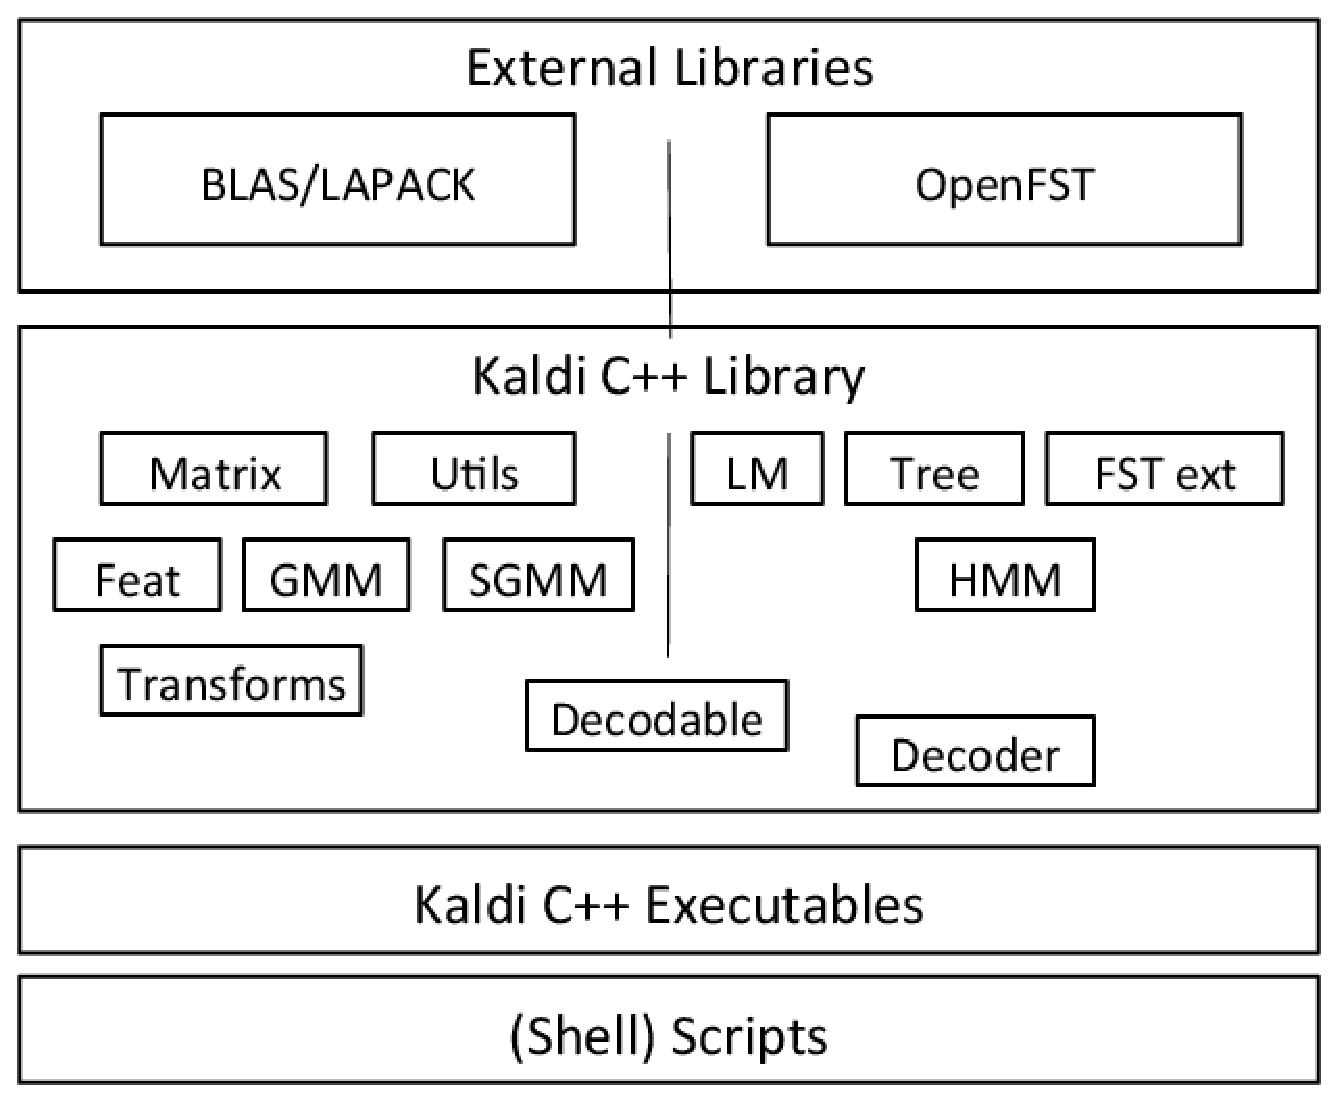
\includegraphics[width=25em]{images/kaldi-lib}
        \caption{Kaldi toolkit architecture\cite{povey2011kaldi}}
        \label{fig:kaldi_arch} 
    \end{center}
\end{figure}

Kaldi uses executables which load its input from files and typically store results again to files.
Alternatively, the~output of one Kaldi program can be feed into next command using system pipes.
There are usually many alternatives for every speech recognition tasks as seen in list of executables below:
\begin{enumerate}
    \item Speech parametrisation
        \begin{itemize}
            \item \term{apply-mfcc}
            \item \term{compute-mfcc-feats}
            \item \term{compute-plp-feats}
            \item \ldots
        \end{itemize}
    \item Feature transformation
        \begin{itemize}
            \item \term{apply-cmvn}
            \item \term{compute-cmvn-stats}
            \item \term{acc-lda}
            \item \term{fmpe-apply-transform}
            \item \ldots
        \end{itemize}
    \item Decoders
        \begin{itemize}
            \item \term{gmm-latgen-faster}
            \item \term{gmm-latgen-faster-parallel}
            \item \term{gmm-latgen-biglm-faster}
            \item \ldots
        \end{itemize}
    \item Evaluation and utilities
        \begin{itemize}
            \item compute-wer
            \item show-alignments
            \item \ldots
        \end{itemize}
\end{enumerate}
In addition, Kaldi provides very useful standardized scripts which wrap Kaldi executables or add new functionality. 
The~scripts are located in \term{utils} and \term{steps} directories and are used in many training scripts recipes for different corpus data.
In this thesis we created a~new training recipe using the~Kaldi infrastructure and Czech and English training corpus \cite{korvas_2014}.
The~recipe, the~data and acoustic modelling scripts are described in~Chapter~\ref{cha:train}.

\subsection{Finite State Transducers} 
\label{sec:fst}
The~\acl{FST} framework and its implementation OpenFST determines the~shape of the~Kaldi data structures.
Kaldi uses \ac{FST} as underlaying representation for \ac{LM}, partially for \ac{AM}, lexicon and also for representing transformation between text, pronunciation and triphones.

The~\ac{FST} framework provides well studied graph operations\cite{mohri2002weighted} which can be effectively used for acoustic modelling.
Using the~\ac{FST} framework the~speech decoding task is expressed as a~beam search in a~graph, which is well studied problem.
% The~OpenFST library implements memory efficient representation of \ac{FST} and provides standardized efficient operations.
% As stated in \cite{mohri2002weighted} and \cite{povey2011kaldi} the~operations can be effectively used for speech decoding. 

The~\ac{FST} graphs used for \ac{AM} model training and speech decoding can be constructed as sequence of standardized OpenFST operations.\cite{mohri2002weighted}.
Decoding is performed on so called \term{decoding graph} $HCLG$ which is constructed from simple \ac{FST} graphs as illustrated in~Equation~\ref{eq:hclg}. 
\begin{equation} \label{eq:hclg}
HCLG = H\circ C\circ L\circ G
\end{equation}.
The~symbol $\circ$ represents an associative binary operation of composition on \acp{FST}.
We briefly explain the~functionality of the~transducers from~Equation~\ref{eq:hclg}:
\begin{enumerate}
    % source  http://kaldi.sourceforge.net/graph.html
    \item G is an acceptor that encodes the~grammar or language model.
    \item L represents the~lexicon. Its input symbols are phones. Its output symbols are words.
    \item C represents the~relationship between context-dependent phones on input and phones on output.
    \item H contains the~\ac{HMM} definitions, that take as input id number of~\acp{PDF} and return context-dependent phones.
\end{enumerate}

Following one liner illustrates how Kaldi decoding graph is created using standard \ac{FST} operations\footnote{Kaldi tutorial on building $HCLG$: \url{http://kaldi.sourceforge.net/graph_recipe_test.html}}.\cite{mohri2002weighted}
\begin{equation}
   HCLG = asl(min(rds(det(H' o min(det(C o min(det(L o G)))))))) 
\end{equation}

\ml{Semiring}
Most of the~operations operate on paths in the~decoding graph.
Path is a~sequence of edges which have weights and an input and an output labels.
Based on the~weight type and weight path operations we distinguish several semirings. 

Formally, a~\term{semiring} $(\mathcal{K}, \oplus, \otimes, \bar{0}, \bar{1})$ is an algebraic structure on set $\mathcal{K}$ with operations $\oplus$ and $\otimes$.
The~binary operations multiplication $\oplus$ and addition $\otimes$ have identity element $\bar{0}$ respectively $\bar{1}$. 
The~$(\mathcal{K}, \oplus)$ forms commutative monoid and $(\mathcal{K}, \otimes)$ forms just a~monoid.
The~multiplication is left and right distributive over addition.
Moreover, multiplication by $\bar{0}$ annihilates any member of $\mathcal{K}$ to $zero$. 
Table~\ref{tab:semiring} shows useful semirings in OpenFST.

\begin{table}[!htp]\label{tab:semiring}
\begin{center}
\begin{tabular}{lrrrrr}
\hline
Name & $\mathcal{K}$ & $\oplus$ & $ \otimes$ & $\bar{0}$ & $\bar{1}$ \\ 
\hline
Real        & $[0,\infty)$        &  +                     &  * &  0        &  1  \\
Log         & $(-\infty, \infty)$ & $-log(e^{-x} + e^{-y})$ & + &  $\infty$ &  0  \\
Tropical    & $(-\infty, \infty)$ &  min                   &  + &  $\infty$ &  0  \\
\hline
\end{tabular}
\caption{Semirings used in speech recognition.\cite{openfst_web}}
\end{center}
\end{table}
